\documentclass[landscape,a0paper,final,showframe]{baposter}

\usepackage{times}
\usepackage{calc}
\usepackage{graphicx}
\usepackage{amsmath}
\usepackage{amssymb}
\usepackage{relsize}
\usepackage{multirow}
\usepackage{bm}

\usepackage{graphicx}
\usepackage{multicol}

\usepackage{pgfbaselayers}
\pgfdeclarelayer{background}
\pgfdeclarelayer{foreground}
\pgfsetlayers{background,main,foreground}

\usepackage{helvet}
%\usepackage{bookman}
\usepackage{palatino}

\newcommand{\captionfont}{\footnotesize}

\selectcolormodel{cmyk}

\graphicspath{{images/}}

%%%%%%%%%%%%%%%%%%%%%%%%%%%%%%%%%%%%%%%%%%%%%%%%%%%%%%%%%%%%%%%%%%%%%%%%%%%%%%%%
%%%% Some math symbols used in the text
%%%%%%%%%%%%%%%%%%%%%%%%%%%%%%%%%%%%%%%%%%%%%%%%%%%%%%%%%%%%%%%%%%%%%%%%%%%%%%%%
% Format 
\newcommand{\Matrix}[1]{\begin{bmatrix} #1 \end{bmatrix}}
\newcommand{\Vector}[1]{\Matrix{#1}}
\newcommand*{\SET}[1]  {\ensuremath{\mathcal{#1}}}
\newcommand*{\MAT}[1]  {\ensuremath{\mathbf{#1}}}
\newcommand*{\VEC}[1]  {\ensuremath{\bm{#1}}}
\newcommand*{\CONST}[1]{\ensuremath{\mathit{#1}}}
\newcommand*{\norm}[1]{\mathopen\| #1 \mathclose\|}% use instead of $\|x\|$
\newcommand*{\abs}[1]{\mathopen| #1 \mathclose|}% use instead of $\|x\|$
\newcommand*{\absLR}[1]{\left| #1 \right|}% use instead of $\|x\|$

\def\norm#1{\mathopen\| #1 \mathclose\|}% use instead of $\|x\|$
\newcommand{\normLR}[1]{\left\| #1 \right\|}% use instead of $\|x\|$

%%%%%%%%%%%%%%%%%%%%%%%%%%%%%%%%%%%%%%%%%%%%%%%%%%%%%%%%%%%%%%%%%%%%%%%%%%%%%%%%
% Multicol Settings
%%%%%%%%%%%%%%%%%%%%%%%%%%%%%%%%%%%%%%%%%%%%%%%%%%%%%%%%%%%%%%%%%%%%%%%%%%%%%%%%
\setlength{\columnsep}{0.7em}
\setlength{\columnseprule}{0mm}


%%%%%%%%%%%%%%%%%%%%%%%%%%%%%%%%%%%%%%%%%%%%%%%%%%%%%%%%%%%%%%%%%%%%%%%%%%%%%%%%
% Save space in lists. Use this after the opening of the list
%%%%%%%%%%%%%%%%%%%%%%%%%%%%%%%%%%%%%%%%%%%%%%%%%%%%%%%%%%%%%%%%%%%%%%%%%%%%%%%%
\newcommand{\compresslist}{%
\setlength{\itemsep}{1pt}%
\setlength{\parskip}{0pt}%
\setlength{\parsep}{0pt}%
}


%%%%%%%%%%%%%%%%%%%%%%%%%%%%%%%%%%%%%%%%%%%%%%%%%%%%%%%%%%%%%%%%%%%%%%%%%%%%%%
%%% Begin of Document
%%%%%%%%%%%%%%%%%%%%%%%%%%%%%%%%%%%%%%%%%%%%%%%%%%%%%%%%%%%%%%%%%%%%%%%%%%%%%%

\begin{document}

%%%%%%%%%%%%%%%%%%%%%%%%%%%%%%%%%%%%%%%%%%%%%%%%%%%%%%%%%%%%%%%%%%%%%%%%%%%%%%
%%% Here starts the poster
%%%---------------------------------------------------------------------------
%%% Format it to your taste with the options
%%%%%%%%%%%%%%%%%%%%%%%%%%%%%%%%%%%%%%%%%%%%%%%%%%%%%%%%%%%%%%%%%%%%%%%%%%%%%%
\typeout{Poster Starts}
\definecolor{silver}{cmyk}{0,0,0,0.3}
\definecolor{yellow}{cmyk}{0,0,0.9,0.0}
\definecolor{reddishyellow}{cmyk}{0,0.22,1.0,0.0}
\definecolor{black}{cmyk}{0,0,0.0,1.0}
\definecolor{darkYellow}{cmyk}{0,0,1.0,0.5}
\definecolor{darkSilver}{cmyk}{0,0,0,0.1}

\definecolor{lightyellow}{cmyk}{0,0,0.3,0.0}
\definecolor{lighteryellow}{cmyk}{0,0,0.1,0.0}
\definecolor{lighteryellow}{cmyk}{0,0,0.1,0.0}
\definecolor{lightestyellow}{cmyk}{0,0,0.05,0.0}

\definecolor{lightblue}{rgb}{0.8,0.8,1}
\definecolor{lighterblue}{rgb}{0.9,0.9,1}
\definecolor{lightestblue}{rgb}{0.98,0.98,1}

\definecolor{cyan}{cmyk}{0.4,0,0.3,0}
\definecolor{greenblue}{rgb}{0.7,1,.7}
\definecolor{mediumblue}{rgb}{0.7,0.7,1}
\begin{poster}{
  % Show grid to help with alignment
  grid=no,
  % Column spacing
  colspacing=1em,
  % Color style
  bgColorOne=lightyellow,
  bgColorTwo=lightestyellow,
  borderColor=mediumblue,
  headerColorOne=lighterblue,
  headerColorTwo=mediumblue,
  headerFontColor=black,
  boxColorOne=lighterblue,
  boxColorTwo=lightblue,
  % Format of textbox
  textborder=roundedleft,
  % Format of text header
  eyecatcher=yes,
  headerborder=open,
  headerheight=0.08\textheight,
  headershape=roundedright,
  headershade=shade-tb,
  headerfont=\Large\textsf, %Sans Serif
  boxshade=plain,
%  background=shade-tb,
  background=shade-tb,
  linewidth=2pt
  }
  % Eye Catcher
  { % The title is centered between eye-catcher and logo.
    \includegraphics[height=5.5em]{figs/cavity-cartoon}
  }
  % Title
  {\sf %Sans Serif
  %\bf% Serif
  A Classical Density Functional for Water}
  % Authors
  {\sf %Sans Serif
  % Serif
  David Roundy\hspace{3em}
  Jessica Hughes\hspace{3em}
  Oregon State University, USA
  }
  % University logo
  {
    
\includegraphics[height=5.5em]{figs/osu-logo}
  }

  \tikzstyle{light shaded}=[top color=baposterBGtwo!30!white,bottom color=baposterBGone!30!white,shading=axis,shading angle=30]

  % Width of left inset image
     \newlength{\leftimgwidth}
     \setlength{\leftimgwidth}{0.78em+8.0em}

%%%%%%%%%%%%%%%%%%%%%%%%%%%%%%%%%%%%%%%%%%%%%%%%%%%%%%%%%%%%%%%%%%%%%%%%%%%%%%
%%% Now define the boxes that make up the poster
%%%---------------------------------------------------------------------------
%%% Each box has a name and can be placed absolutely or relatively.
%%% The only inconvenience is that you can only specify a relative position 
%%% towards an already declared box. So if you have a box attached to the 
%%% bottom, one to the top and a third one which should be in between, you 
%%% have to specify the top and bottom boxes before you specify the middle 
%%% box.
%%%%%%%%%%%%%%%%%%%%%%%%%%%%%%%%%%%%%%%%%%%%%%%%%%%%%%%%%%%%%%%%%%%%%%%%%%%%%%
    %
    % A coloured circle useful as a bullet with an adjustably strong filling
    \newcommand{\colouredcircle}[1]{%
      \tikz{\useasboundingbox (-0.2em,-0.32em) rectangle(0.2em,0.32em); \draw[draw=black,fill=baposterBGone!80!black!#1!white,line width=0.03em] (0,0) circle(0.18em);}}

  \headerbox{Classical DFT}{name=cdft,column=0,row=0}{ Classical
    Density-Functional Theory is a continuum empirical approach to
    modelling fluid behavior when the density is inhomogeneous---as is
    the case at interfaces.  We have developed a classical density
    functional for water, which provides a description of hydrophobic
    interactions.

    \vspace{1em}
  }

  \headerbox{Statistical Associating Fluid
    Teory}{name=saft,column=0,below=cdft}{ Statistical Associating
    Fluid Theory (SAFT) is a well-established approach for the
    description of the thermodynamics and phase equilibria of fluid
    systems, with particular applicability to hydrogen-bonding fluids.
    Our functional is constructed so as to reduce in the homogeneous
    limit to the 4-site SAFT model for water developed in
    reference~\cite{clark2006developing}.
    \begin{center}
      \includegraphics[width=\columnwidth]{figs/pressure-with-isotherms}
    \end{center}
    This functional accurately describes the liquid-vapor phase
    diagram away from the critical point, but gives less accurately
    describes the compressibility.

    \vspace{1em}
  }

  \headerbox{The Functional}{name=functional,column=1,row=0}{
    The Helmholtz free energy of the new functional is based on SAFT,
    and is composed of the usual terms:
    \begin{equation*}
      F[n] = F_\textit{id}[n] + F_\textit{hs}[n] + F_\textit{assoc}[n] + F_\textit{disp}[n],
    \end{equation*}
    We model the repulsive interactions using the White Bear version
    of the Fundamental-Measure Theory~(FMT)
    functional~\cite{roth2002whitebear} for the hard sphere fluid,
    which is expressed in terms of efficiently-computable
    convolutions.
    \vspace{0.5em}

    The SAFT free energy of association for a 4-site model of water
    has the form
    \begin{align*}
      f_\text{assoc} &= 4 k_BT n \left(\ln X - \frac{X}{2} + \frac12\right)
    \end{align*}
    where $X$ is the fraction of hydrogens \emph{not} hydrogen bonded,
    and is found using a mass action equation involving the density of
    hard spheres in contact with one another.  We extend this to the
    inhomogeneous case using the approach described by Yu and
    Wu~\cite{yu2002fmt-dft-inhomogeneous-associating}, which expresses
    $X$ in terms of the same weighted densities used in FMT.
    \vspace{0.5em}

    Finally, we add a simple and efficient functional for the
    dispersion interaction based on
    SAFT-VR~\cite{gil-villegas-1997-SAFT-VR}, with an additional
    tunable parameter to adjust the surface tension.

    \vspace{0.8em}
  }

  \headerbox{Surface
    Tension}{name=surfacetension,column=1,below=functional,above=bottom}{
    We compute the surface tension by finding the free energy of a
    liquid-vapor interface.  The surface tension is fit to experiment
    by adjusting a length-scale parameter in the dispersion term of
    the free energy.
    \begin{center}
      \includegraphics[width=\columnwidth]{figs/surface-tension}
    \end{center}
  }
  \headerbox{A Single Cylinder in Water}{name=rod,column=2,span=2,row=0}{
    \begin{multicols}{2}
      One of the simplest multi-dimensional inhomogeneous systems is a
      hard cylinder in water.
      \begin{center}
        \includegraphics[width=0.9\columnwidth]{figs/density-vs-radius}
      \end{center}
      \begin{quote}
        The density of water around a
        hard-walled cylinder with 1~nm diameter.
      \end{quote}

      \begin{center}
        \includegraphics[width=\columnwidth]{figs/energy-vs-diameter}
      \end{center}
      \begin{quote}
        The hydration energy per unit area of a hard
        cylinder.  As expected, this asymptotes to the same value as
        the surface tension.
      \end{quote}
    \end{multicols}
  }
  \headerbox{Two Cylinders in Water}{name=two rods,column=2,span=2,below=rod,above=bottom}{
    %% \begin{multicols}{2}
    %%   This text will be in two separate columns.
    %%   This text will be in two separate columns.
    %%   This text will be in two separate columns.
    %%   This text will be in two separate columns.
    %%   This text will be in two separate columns.
    %%   This text will be in two separate columns.
    %%   This text will be in two separate columns.
    %% \end{multicols}\vspace{-1em}
    \begin{multicols}{2}
      \includegraphics[width=\columnwidth]{figs/density-rods-in-water}

      \vspace{-1em}
      \begin{quote}
        The density of water in the vicinity of two hard-walled
        cylinders, each 1~nm in diameter, and separated by 1~nm.
      \end{quote}

      \includegraphics[width=\columnwidth]{figs/xassoc-rods-in-water}

      \vspace{-1em}
      \begin{quote}
      Here we plot the number of hydrogen bonds per molecule for the
      same system of two hard-walled cylinders.
      \end{quote}
    \end{multicols}
    
    \begin{multicols}{2}
      One application of our model is the hydrophobic attraction
      between two cylindrical molecules in water, such as two
      nanotubes.  We study the interactions between two hard cylinders
      with 1~nm diameter.
      \begin{center}
        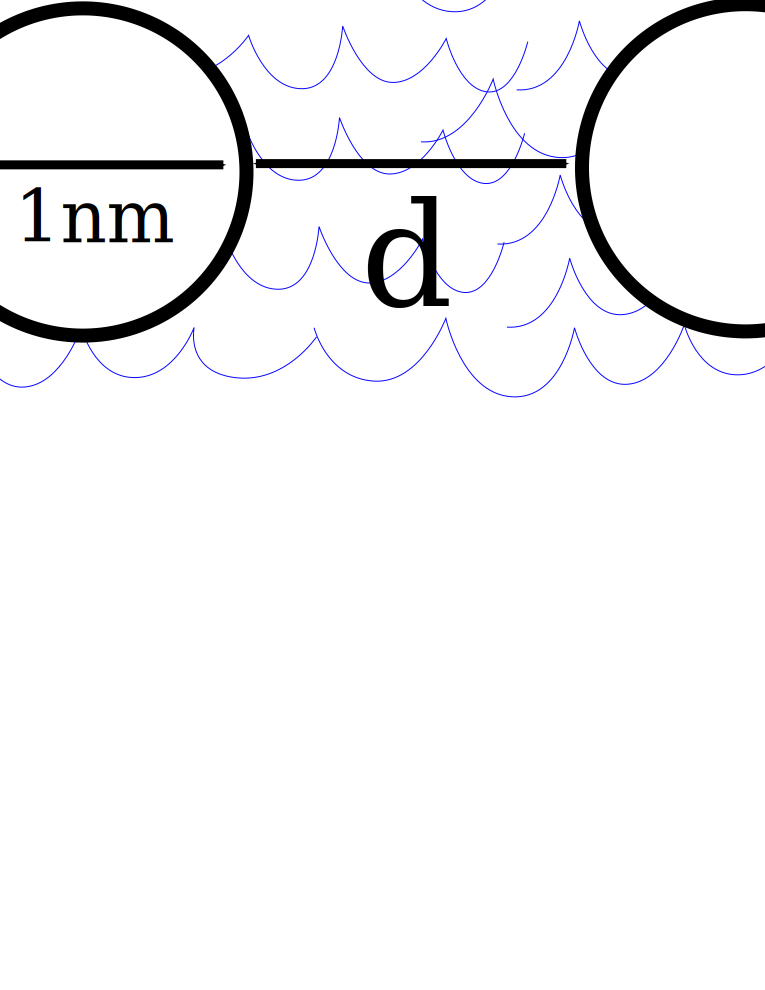
\includegraphics[width=0.95\columnwidth]{figs/two-rods-diagram}
      \end{center}
      \begin{center}
        \includegraphics[width=0.9\columnwidth]{figs/rods-energy-vs-distance}
      \end{center}
    \end{multicols}
  }%
  %% \headerbox{Future Work}{name=future work,column=3,span=1,above=two rods,row=0}{
  %%   \begin{itemize}
  %%   \item Extend functional to depend on hydrogen and oxygen densities
  %%     separately, including intramolecular interactions in the
  %%     harmonic approximation.
  %%   \item Introduce elecrtrostatic interactions.
  %%   \item Couple with.
  %%   \end{itemize}
  %% }
  \headerbox{References}{name=references,column=0,above=bottom,below=saft}{
    \renewcommand\refname{}
    \bibliographystyle{unsrt}
    \tiny
    \bibliography{paper}
  }%
\end{poster}%
%
\end{document}
